\chapter{Realisierung}

\section{Systemübersicht}

\begin{figure}[H]
	\centering
	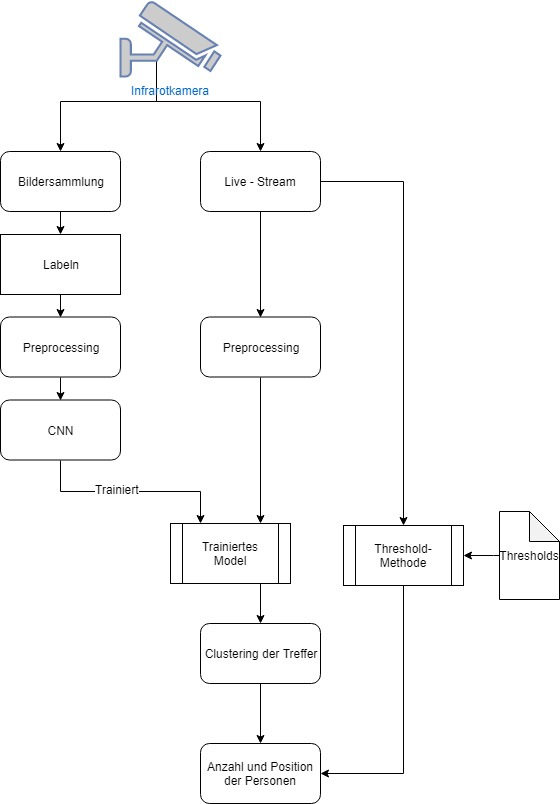
\includegraphics[width=.7\linewidth]{SystemOverview}
	\caption{Grobübersicht des Systems mit CNN- und Thresholdalgorithmus}
	\label{SystemOverview}
\end{figure}

\section{UDP-Schnittstelle}

Um die Bilder automatisiert erhalten zu können wurde eine Schnittstelle zu den Infrarotkameras implementiert. Es wurde das UDP-Protokoll verwendet, da die Kameras nur über dieses Protokoll angesprochen werden konnten.\\
 Die einzige ander Möglichkeit and Bilder zu gelangen wäre über die GUI Applikation des Herstellers Videos aufzunehmen. Dies sind bereits auf RGB convertiert, beihalten also nicht alle Information des ursprünglichen Bildes und die Applikation kann nicht automatisiert angesprochen werden. Folglich ist dies keine praktikable Variante um effizient Daten zu sammeln.\\
\\
Die Kameras können ausserdem nur mittels UDP-Broadcasts identifiziert und and einen Socket gebunden werden. Aus diesem Grund konnten die Kameras nicht im allgemeinen Schulnetzwerk installiert werden, sondern mussten in einem separaten Netzwerk betrieben werden. In diesem Netzwerk konnten sie über einen Computer angesteuert werden, der widerum mit dem HSLU-Netzwerk verbunden ist. Um die Entwicklung der Schnittstelle möglichst einfach zu gestalten wurde versucht einen Remoteinterpreter aufzusetzen. Dies ist eine funktion von Pycharm \parencite{pycharm} erlaubt es, auf einem Lokalen System zu entwickeln aber die Software direkt auf einem Remote System auszuführen und zu Debuggen.\\
Leider wird dies für Windows Remote Systeme nicht unterstützt. Deshalb wurde der Code jeweils manuell via sftp auf den Computer im Sitzungszimmer kopiert. Danach wurde mittel Windows Remotedesktopverbindung die Software ausgeführt und getestet. \\
\\
In einer ersten Variante wurde in dieser Schnittstelle mit Einzelbilder gearbeitet. Dies bietet den Vorteil, dass man die Bildrate einfah definieren und steuern kann. Leider war die Qualitiät dieser Bilder sehr schlecht. Durch eine Rücksprach mit dem Hersteller stellte sich heraus, das die Verwendung der Streaming Funktion der Kameras qualitativ besser Bilder liefert. Deshalb wurde die Schnittstelle auf die Verwendung von Streams abgeändert. Dabei war die Generator Funktionalität von Python sehr hilfreich. Die Eigenschaft von Generators, dass diese erst ausgeführt werden, wenn ein Objekt angefragt wird, konnte genutzt werden, um jederzeit das aktuellste Bild zu erhalten.

\section{Datensammlung}

Um die Trainingsdaten effizient zu sammeln wurde ein  Skript erstellt, welches von beiden Kameras gleichzeitig Bilder anfordert und Abspeichert. Dieses musste über mehrere Monate unterbruchlos laufen und wurde deshalb so Implementiert, dass es sich bei einem Fehler automatisch neu startet. Zusätzlich wurden parallel dazu auch Bilder der Referenzkamera aufgezeichnet, um das Labeling der Infrarotbilder zu vereinfachen und als Ground Truth zu verifizieren.\\
Alle aufgezeichneten Bilder wurden lokal auf einer Festplatte des Computers im Sitzungszimmer gespeichert. Um alle Bilder eindeutig zu identifizieren, wurden sie mit Art des Bildes, Infrarot oder Ground Truth, Zeitstempel und bei den Infrarotbildern mit Kamera 1 oder 2 versehen. Um das ganze übersichtlicher zu gestalten wurde das ganze in einem Ordnersystem abgelegt, das wie folgt aufgebaut ist.

\begin{itemize}[leftmargin=4cm, align=left, labelsep=*, labelwidth=*]
	\item[Ordnerschema] ../ [Jahr] / [Monat] / [Tag] / [Bildtyp]\_[Uhrzeit]\_[Kamera].[Dateityp]
	\item[Beispiel] ../2019/05/23/IR\_Image\_10\_33\_45\_2.npy
\end{itemize}


\section{CNN}

Um das \gls{CNN} trainieren zu können müssen die Bilder gelabelt, \gls{Padding} hinzugefügt, \glspl{Window} extrahiert, und normalisiert werden. Dazu wurden verschiedene Module implementiert, die diese Aufgaben übernehmen.

\subsection{Labeln}
\label{sec:labeling}

Für das Labeln der Bilder wurde \textit{labelme}\parencite{labelme2016} verwendet da dies einfaches und praktisches User Interface bietet. Die Labels wurden jeweils in dem Verzeichnis \textit{labels} abgelegt, der auf der gleichen ebene wie das Verzeichnis \textit{ir\_images} in dem die dazugehörigen Infrarotbilder abgelegt sind.\\
Die rohen Infrarotbilder wurden als .npy-Dateien gespeichert \parencite{npyformat}. Dies, weil die Pixelwerte der Bilder in Kelvin*10 sind, d.h. 2731 entspricht 0\degree C. Aus diesem Grund konnten sie nicht auf einfache Art in ein Grafikformat persistiert werden. Zudem ist es wünschenswert Berechnungen mit den Originalwerten durchzuführen.\\
Um die Infrarotbilder aber labeln zu können wird ein Bild mit .jpg oder ähnlichem Format benötigt. Dazu wurde das Bild auf Graustufen reduziert. Dabei geht zwar ein Teil der Information verloren, aber man kann genug erkennen um die Bilder korrekt zu Labeln. zudem konnte im Zweifelsfall das RGB Bild der Referenzkamera zu Hilfe gezogen werden. Da die konvertierten Bilder die gleichen Dimensionen aufweisen können die definierten Labels direkt auf die Infrarotbilder angewendet werden.

\subsection{Preprocessing der Trainingsdaten}

Um das vorbereiten der Trainigsdaten möglichst einfach zu gestalten wurde die Klasse Loader implementiert. Dies bietet die Methode \textit{load\_data\_by\_labels}, welche für ein spezifiziertes Verzeichnis alle Objekte lädt für die ein Label existiert. Diese Methode basiert darauf das die Labels und Infrarotbildern wie vorgängig erwähnt im selben Verzeichnis und in den Ordnern \textit{labels} und \textit{ir\_images} abgelegt wurden. Die Methode kann zudem mit mehreren Parameter angepasst weden.

\subsubsection{Loader}

\noindent -Konstruktor Parameter:
\begin{itemize}[leftmargin=*, labelindent=3cm, labelsep=1cm]
	\item[\textit{source\_folder}] String: Das Verzeichnis aus dem die Trainingsdaten geladen werden sollen, muss die Ordner \textit{ir\_images} und \textit{labels} beinhalten.
	\item[\textit{window\_size}] (int, int): Die grösse des Fensters das um das Label extrahiert werden soll.
	\item[\textit{extend\_by\_roaming}] Boolean: Um jedes Label wird in einem Umkreis drei Pixeln zusätzliche Fenster extrahiert. Dies ist eine Methode um mehr trainigsdaten zu generieren und das CNN darauf zu trainieren die Objekte nicht nur zentriert zu erkennen.
\end{itemize}
\vspace{2em}
\noindent\textit{load\_data\_by\_labels()} Parameter:
\begin{itemize}[leftmargin=*,labelindent=3cm, labelsep=1cm]
		\item[\textit{cam}] Int: 1 oder 2 von welcher der Kameras die Bilder geladen werden sollen. Wird dieser Parameter nicht verwendet werden Bilder beider Kameras verwendet.
		\item[\textit{no\_background}] Boolean: Es werden soviele, zufällig ausgewählte Hintergrundausschnitte aus einem Referenzbild geladen wie die negativ Klasse enthält, wenn True.
		\item[\textit{rotate\_negatives}] Boolean: rotiert alle Fenster der negativ Klasse 3 mal um 90\degree und spiegelt sie, wenn True.
		\item[\textit{rotate\_positives}] Boolean: rotiert alle Fenster der positiv Klasse 3 mal um 90\degree und spiegelt sie, wenn True.
\end{itemize}

\noindent mit diesen Möglichkeiten können die Daten in zwei Zeilen Code individuell für jedes Training vorbereitet werden.\\
\\
Vor dem Training werden die Daten dann zusätzlich noch normalisiert, damit alle Werte zwischen 0 und 1 liegen und das Datenset wird gemischt, dass beim Training nicht ganze Batches dieselbe Klasse repräsentieren.

\subsection{Aufbau des CNN}

Es wurden Verschiedene \gls{CNN} Architekturen getestet. Zu Beginn wurde versucht einen Binär Klassifizierer zu entwickeln. Da aber die Negativklasse zu viele verschieden Objekte beinhaltete wurde entschieden mit drei Klassen zu arbeiten, \textit{Person}, \textit{Fremde Wärmequellen} und \textit{Hintergrund}. Diese Version erzeugte erstmals akzeptable Resultate. Daraufhin wurde weiter getestet und recherchiert um das Modell zusätzlich zu optimieren. Aufgrund dieser recherche wurde Das \gls{CNN} nach dem Vorbild des LR-CNN \parencite{cnnArchitecture} aufgebaut, da auch diese Arbeit sich auf Bilder mit niedriger Auflösung spezialisiert. Das verwendete CNN sieht wie folgt aus:

% Tabelle mit ergebnissen
{
	\renewcommand{\arraystretch}{1.3}
	
	\begin{table}[H]
		\scriptsize
		\centering
		\begin{tabularx}{.8\textwidth}{XX}\\
			\multicolumn{2}{c}{\textbf{CNN Architektur}}\\
			\hline
			\textbf{Layers} & \textbf{Attribute}\\
			\hline
			\textit{Convolutional Layer} & 64 5x5 Filter RelU Activation mit Padding\\
			\hline
			\textit{MaxPooling} & 3x3 Stride=(2,2)\\
			\hline 
			\textit{Convolutional Layer} & 64 5x5 Filter RelU Activation mit Padding\\
			\hline
			\textit{MaxPooling} & 3x3 Stride=(2,2)\\
			\hline
			\textit{Convolutional Layer} & 64 3x3 Filter RelU Activation mit Padding\\
			\hline
			\textit{MaxPooling} & 3x3 Stride=(2,2)\\
			\hline
			\textit{Fully Connected Dense Layer} & Outputsize 128 RelU Activation\\
			\hline
			\textit{Dropout} & 0.5\\
			\hline
			\textit{Fully Connected Dense Layer} & Outputsize 3 Softmax Activation\\
			\hline
		\end{tabularx}
		\caption{Architektur des Finalen CNN}
		\label{tbl:cnnArchitecture}
	\end{table}
	\begin{table}[H]
		\scriptsize
		\centering
		\begin{tabularx}{.8\textwidth}{XX}
			\multicolumn{2}{c}{\textbf{CNN Hyperparameter}}\\
			\hline
			\textbf{Parameter} &  \textbf{Wert}\\
			\hline
			\textit{Window Size} & 16x16\\
			\hline
			\textit{Optimizer} & Adam\\
			\hline  
			\textit{Loss} & Categorical Crossentropy\\
			\hline
			\textit{Metric} & Categorical Accuracy\\
			\hline
			\textit{Batchsize} & 32\\
			\hline
			\textit{Epochen} & 7\\
			\hline
		\end{tabularx}
		\caption{Hyperparameter des Finalen CNN}
		\label{tbl:hyperparameter}
	\end{table}
}


\noindent Die Funktionsweise des Maxpooling ist in Abbildung \ref{fig:maxpoolSample} dargestellt. Es wird von jedem Feld jeweils der grösste Wert ausgewählt und daraus das neue Bild zusammengesetzt.

\begin{figure}[H]
	\centering
	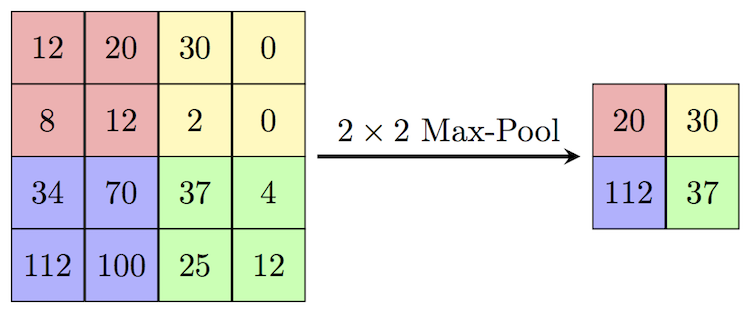
\includegraphics[width=.5\linewidth]{MaxpoolSample}
	\caption{Visualisierung Maxpooling \parencite{MaxpoolImg2018}}
	\label{fig:maxpoolSample}
\end{figure}

\begin{figure}[H]
	\centering
	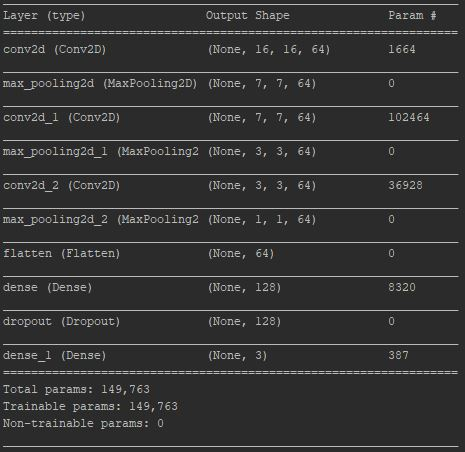
\includegraphics[width=.7\linewidth]{modelSummary}
	\caption{Architektur des CNN}
	\label{fig:cnnArchitecture}
\end{figure}

\subsection{Training}

Für das training wurden x Auschnitte aus x Bildern verwendet. Diese wurden Rotiert und Gespiegelt. Für die Negativklasse wurde zusätzlich Roaming eingesetzt, Dies weil auf diese Art Randgebiete von Wärmequellen eher als kein Treffer gewertet werden. Insgesamt wurden auf diese Weise 7323 Trainingsbilder erzeugt. Mit denen das \gls{CNN} trainiert werden konnte. Für die Grösse des Bildausschnitts wurde ein 16x16 Fenster verwendet, da dieses gross genug ist um im Normalfalls eine ganze Person zu beinhalten aber auch klein genug um nur eine einzelne Person zu umschliessen.

\subsection{Anwendung des Trainierten Modells}

Um nun ein Bild zu analysieren und zu bestimmen, an welchen Positionen sich die Personen im Bild befinden, wurde die Klasse \textit{People\_Finder} implementiert. Diese bietet nach aussen die Methode \textit{find\_people(image)} an. Diese Methode returniert die Treffer und deren Position.\\
In dieser Methode wird das Bild mit \gls{Padding} und in \glspl{Window} unterteilt, diese werden dann mit dem \gls{CNN} ausgewertet. Wird ein \gls{Window} als Person markiert, wird das Zentrum des \glspl{Window} gespeichert. Um mehrere Treffer auf derselben Person zu verhindern werden abschliessend alle Treffer zu \gls{Cluster} zusammengefasst. So werden Treffer die direkt nebeneinander liegen zu einem einzelnen Treffer zusammengeführt.

\section{Threshold-Methode}

Die Threshold-Methode wurde zu Beginn so implementiert, dass mit verschiedenen Schieberegler die Parameter festgelegt werden konnten. Diese Methode vereinfachte das Finden von passenden Parameter enorm. Die finale Version der Threshold-Methode nimmt ein \textit{Threshold} Datenobjekt als Parameter entgegen. So können die Parameter angepasst werden ohne, dass die Implementation geändert werden muss.\\
Die Folgenden Thresholds wurden verwendet:

% Tabelle mit ergebnissen
{
	\renewcommand{\arraystretch}{1.3}

	\begin{table}[H]
		\scriptsize
		\centering
		\begin{tabularx}{.6\textwidth}{XX}\\
			\multicolumn{2}{c}{\textbf{Thresholds}}\\
			\hline
			\textbf{Typ} & \textbf{Wert}\\
			\hline
			\textit{Minimaltemperatur} & 297.7 K\\
			\hline
			\textit{Maximaltemperatur} & 305.1 K\\
			\hline 
			\textit{Horizontal \gls{Erode}} & 6 Mal mit 3x6 Kernel\\
			\hline
			\textit{Horizontal \gls{Dilate}} & 9 Mal mit 3x6 Kernel\\
			\hline
			\textit{Vertical \gls{Erode}} & 6 Mal mit 6x3 Kernel\\
			\hline
			\textit{Vertical \gls{Dilate}} & 9  Mal mit 6x3 Kernel\\
			\hline
		\end{tabularx}
		\caption{Thresholdwerte}
		\label{tbl:thresholds}
	\end{table}
}

\noindent
Bei der Verarbeitung wird das Infrarotbild zuerst um Faktor 10 vergrössert, da die Kernel sonst zu gross wären. Danach werden alle Pixel, die zwischen Minimal- und Maximaltemperatur liegen, auf den Wert 255 (Weiss) und alle übrigen auf den Wert 0 (Schwarz) gesetzt. Auf das resultierende Bild wird zuerst horizontal und danach vertikal, \gls{Erode} und \gls{Dilate} angewendet. Auf dem daraus resultierenden Binärbild werden nun mittels der OpenCV-Funktion \textit{find\_contours()} die Zentren aller geschlossenen weissen Flächen bestimmt. Diese Zentren entsprechen der Position der Personen.


\section{Evaluationssystem}

Damit die Evaluation simpel und effizient durchgeführt werden konnte, wurde ein System zur automatisierten Testauswertung implementiert. Dazu wurde eine spezifische Ordnerstruktur aufgebaut, nach folgendem Schema:

\begin{itemize}[leftmargin=4cm, align=left, labelsep=*, labelwidth=*]
	\item[Ordnerschema] ../ Experimente / [Experimentgruppe] / [Experimentname] /
	\item[Beispiel] ../Experimente / distance / 20cm / 
\end{itemize}

\noindent
Im untersten Verzeichnis müssen die beiden Ordner, \textit{/ir\_images/} und \textit{/labels/}, enthalten sein. Bei der Auswertung der Experimente wird zu jeder .json-Datei in \textit{/labels/} das passende Infrarotbild aus \textit{/ir\_images/} geladen und mittels dem zu testenden Algorithmus ausgewertet. Die Resultate des Algorithmus werden daraufhin in der \textit{Validator} Klasse mit den Labels verglichen. Dabei werden True Positive, False Positive, False Negative sowie der Mean Squared Error der Treffer zu den Labels ermittelt. Diese Daten werden als \textit{Score} Objekt retourniert.\\

\subsection{Klassen}

In den folgenden Abschnitten verwendete Fachbegriffe werden im Kapitel \ref{sec:explanation} erklärt.

\subsubsection{Score}

\begin{itemize}[leftmargin=*,labelindent=3cm, labelsep=1cm]
	\item[\textit{print()}] Erstellt eine Zusammenfassung der Ergebnisse und zeigt diese in der Konsole
	\item[\textit{draw\_on(image)}] Zeichnet True Positive, False Positive und False Negative auf das übergebene Bild.
\end{itemize}

\noindent
Um die Ergebnisse mehrere Bilder oder Experimente zusammenfassen und visualisieren zu können. Wurde die \textit{Summary} Klasse erstellt. Die \textit{Summary} Klasse bietet die Möglichkeit mehrere \textit{Score} Objekte zusammenzufassen. Zudem können beliebig viele \textit{Summary}'s zusammengeführt werden.

\subsubsection{Summary}

\begin{itemize}[leftmargin=*,labelindent=3cm, labelsep=1cm]
	\item[\textit{print()}] Erstellt eine Zusammenfassung der Ergebnisse und zeigt diese in der Konsole
	\item[\textit{get\_accuracy()}] Berechnet die Accuracy über alle Ergebnisse
	\item[\textit{get\_precision()}] Berechnet die Precision über alle Ergebnisse
	\item[\textit{get\_recall()}] Berechnet den Recall über alle Ergebnisse
	\item[\textit{get\_f1\_score()}] Berechnet die F1-Score über alle Ergebnisse
	\item[append\_summary()] Fügt ein weiteres \textit{Summary} Objekt dieser \textit{Summary} hinzu
\end{itemize}

\subsection{Auswertung}

Um nun die Experimente auszuwerten wurde das \textit{validate\_experiments} Skript implementiert. Dieses iteriert über alle Experimente und führt für jedes die \textit{Validator.validate()} Methode aus. Danach werden die Resultate der einzelnen Experimente und eine Zusammenfassung aller Resultate auf der Konsole ausgegeben. Zusätzlich bietet dieses Skript die Möglichkeit die Resultate jedes Bildes einzuzeichnen und diese anzuzeigen oder direkt in dem zum Experiment gehörenden Verzeichnis als .jpg-Datei abzuspeichern.
